%
% Cura.tex
%
% LulzBot Mini User Manual
%
% Copyright (C) 2014 Aleph Objects, Inc.
%
% This document is licensed under the Creative Commons Attribution 4.0
% International Public License (CC BY-SA 4.0) by Aleph Objects, Inc.
%

\section{Cura}
\index{Cura}

\subsection{Setup Cura}
\index{Installation}

Cura is available for download on our website at \texttt{https://www.lulzbot.com/support/downloads}. When first opening Cura, you will be prompted to go through the \texttt{First time run wizard}. This will consist of selecting your desired language, and your printer.

\textcolor{red}{It is important to select the correct printer, as Cura uses custom profiles and machines settings based upon which printer you are running.}

\begin{itemize}
\item Download the appropriate installer for your computer operating system.
\item Install Cura by clicking on the installer.
\item Once your language has been selected, select \texttt{Next}.
\item Select \texttt{Lulzbot Mini}. 
\item Once the proper printer is selected, select \texttt{Next}. 
\end{itemize}

Once the installation wizard finishes you can move forward with your first print!


\section{Quick Print Settings}
\index{Quick Print Settings}
%\pageref{fig:Cura}.
\begin{figure}[hbt]
\centering
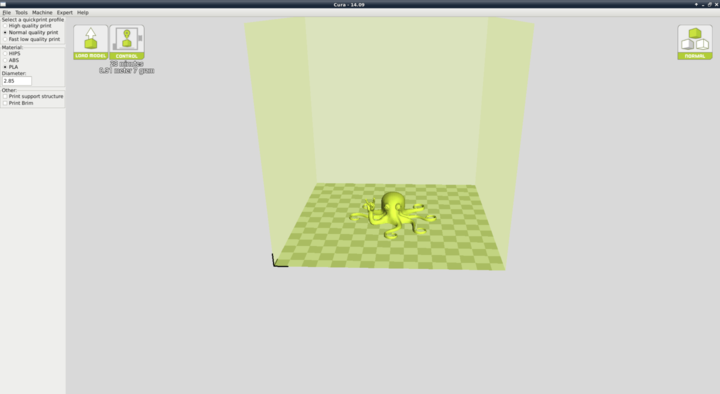
\includegraphics[keepaspectratio=true,angle=0,height=0.4\textheight,width=1.0\textwidth]{Quick_Settings.png}
\caption{Quick Print Settings}
\label{fig:Cura}
\end{figure} 
% (photo highlighting profile, material, diameter, and other)
After setting up Cura for the first time, you will be prompted with this screen (Fig. \ref{fig:Cura}, page \pageref{fig:Cura}: 

\subsection{Selecting a Quick Print Profile}
\index{Quick Print Profile}
\index{Resolution}
In the top left hand corner are the print quality settings. For most filaments, there will be a High Quality, Normal Quality, or Fast Quality options. Some of the more exotic filaments may only have a normal setting.

\subsection{High Quality}
\index{High Quality}

This setting is designed to give greater detail and finer objects. This will have a smaller layer height, which will make each layer thinner, so that curves seem more natural and walls seem less noticable. This setting will also require more layers to be laid down, increasing overall print time.

\subsection{Medium Quality}
\index{Medium Quality}

This setting is designed to give a medium resolution, by increasing the layer height and print speeds. This will make the organic curves slightly more step-like than the fine setting, but will reduce overall print time. 

\subsection{Fast Quality}
\index{Fast Quality}

This setting is designed for the fast prints, where overall model finish is not of concern. Most commonly used for quick iteration of designs for rapid prototyping.

\subsection{Material Selection}
\index{Material Selection}
\index{filament}

Choose your desired filament. If you are not using Lulzbot supplied filament, you will want to update your filament diameter to your specific average filament diameter. You can do this by taking a dozen filament diameter measurements from different parts of the reel and averaging them. Update your filament diameter. You may also want to adjust the temperature, as different manufacturers have different recommended temperatures.

\subsection{Print Support Structure}
\index{Support}
\index{Support Material}

%%%% Saved for standalone Cura Manual %%%%
%The TAZ and TAZ Mini is able to print models that have angles and overhangs, even without support material depending on the overhang distance and angle. Turn this option on if your model requires support material.
The Mini is able to print models that have angles and overhangs, even without support material depending on the overhang distance and angle. Turn this option on if your model requires support material.

\subsection{Brim}
\index{Brim}

Brim is used to increase surface area of the part your printing, thereby ensuring proper part adhesion. This will put down a single layer around the outside of the part, helping first layer adhesion and minimizing warping.

\subsection{Load Model File}
\index{Load Model}
\index{STL}

Select the model you would like to print. Either use the \texttt{Load Model} button or select \texttt{File} > \texttt{Load Model}. Once the file has been loaded, you will see a 3D rendering of your object on the build platform. Select the model to see the various options. 

\subsection{Orientation of STL}
\index{Orientation}

%\pageref{fig:Options}).
\begin{figure}[hbt]
\centering
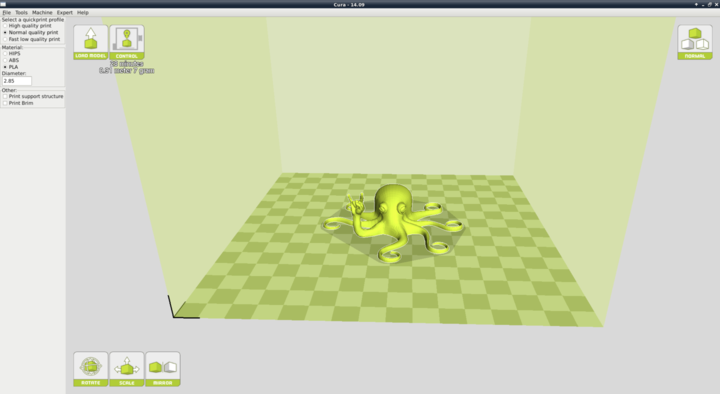
\includegraphics[keepaspectratio=true,angle=0,height=0.4\textheight,width=1.0\textwidth]{Options.png}
\caption{Options after selecting model}
\label{fig:Orientation}
\end{figure}

Move your model to change where it is printed on the build plate. Do this by clicking and dragging your model to the desired location. The \texttt{black} outlined corner represents the lower left hand corner of the build plate on your printer. 


%\pageref{fig:Rotating}).
\begin{figure}[hbt]
\centering
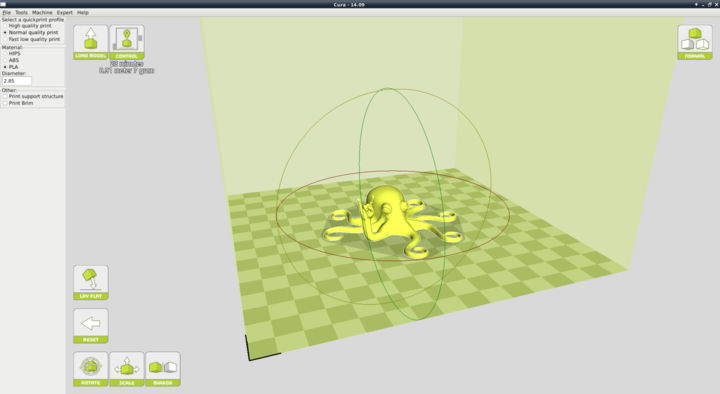
\includegraphics[keepaspectratio=true,angle=0,height=0.4\textheight,width=1.0\textwidth]{Rotate.png}
\caption{Rotating your Model}
\label{fig:Rotating your Model}
\end{figure}

%%%% Alternate explanation %%%%
%The \texttt{Rotate} button will give you the ability orient your model in along all three axes. Once you click the rotate button, three circles will surround your model. The red circle will allow you to rotate in the XY plane. The Yellow circle will rotate in the XZ plane. The Green circle will rotate in the YZ plane.

The \texttt{Rotate} button will give you the ability orient your model in along all three axes. Once you click the rotate button, three circles will surround your model. The \textcolor{red}{red} circle will allow you to rotate around the \textcolor{red}{Z axis}. The \textcolor{yellow}{Yellow} circle will rotate around the \textcolor{yellow}{Y axis}. The \textcolor{green}{Green} circle will rotate around the \textcolor{green}{X axis}.

The \texttt{Lay Flat} button will ensure that the flat portion of your print is securely attached to the bed. It is highly recommended to use this option after rotating your model in the Z direction, as it will help prevent adhesion issues during the print.

The \texttt{Reset} button will return your model to the original orientation as defined by the CAD program used to create the model. 

The Scale button will give you complete dimensions, along with the ability to scale in the X Y or Z directions. As a default, it will be set to uniform scaling. This will cause the X Y and Z axis to be scaled by the same amount, when you make a change to any of them. To disable this, please click the lock in the lower section of the scaling window. 

%\pageref{fig:Scaling}).
\begin{figure}[hbt]
\centering
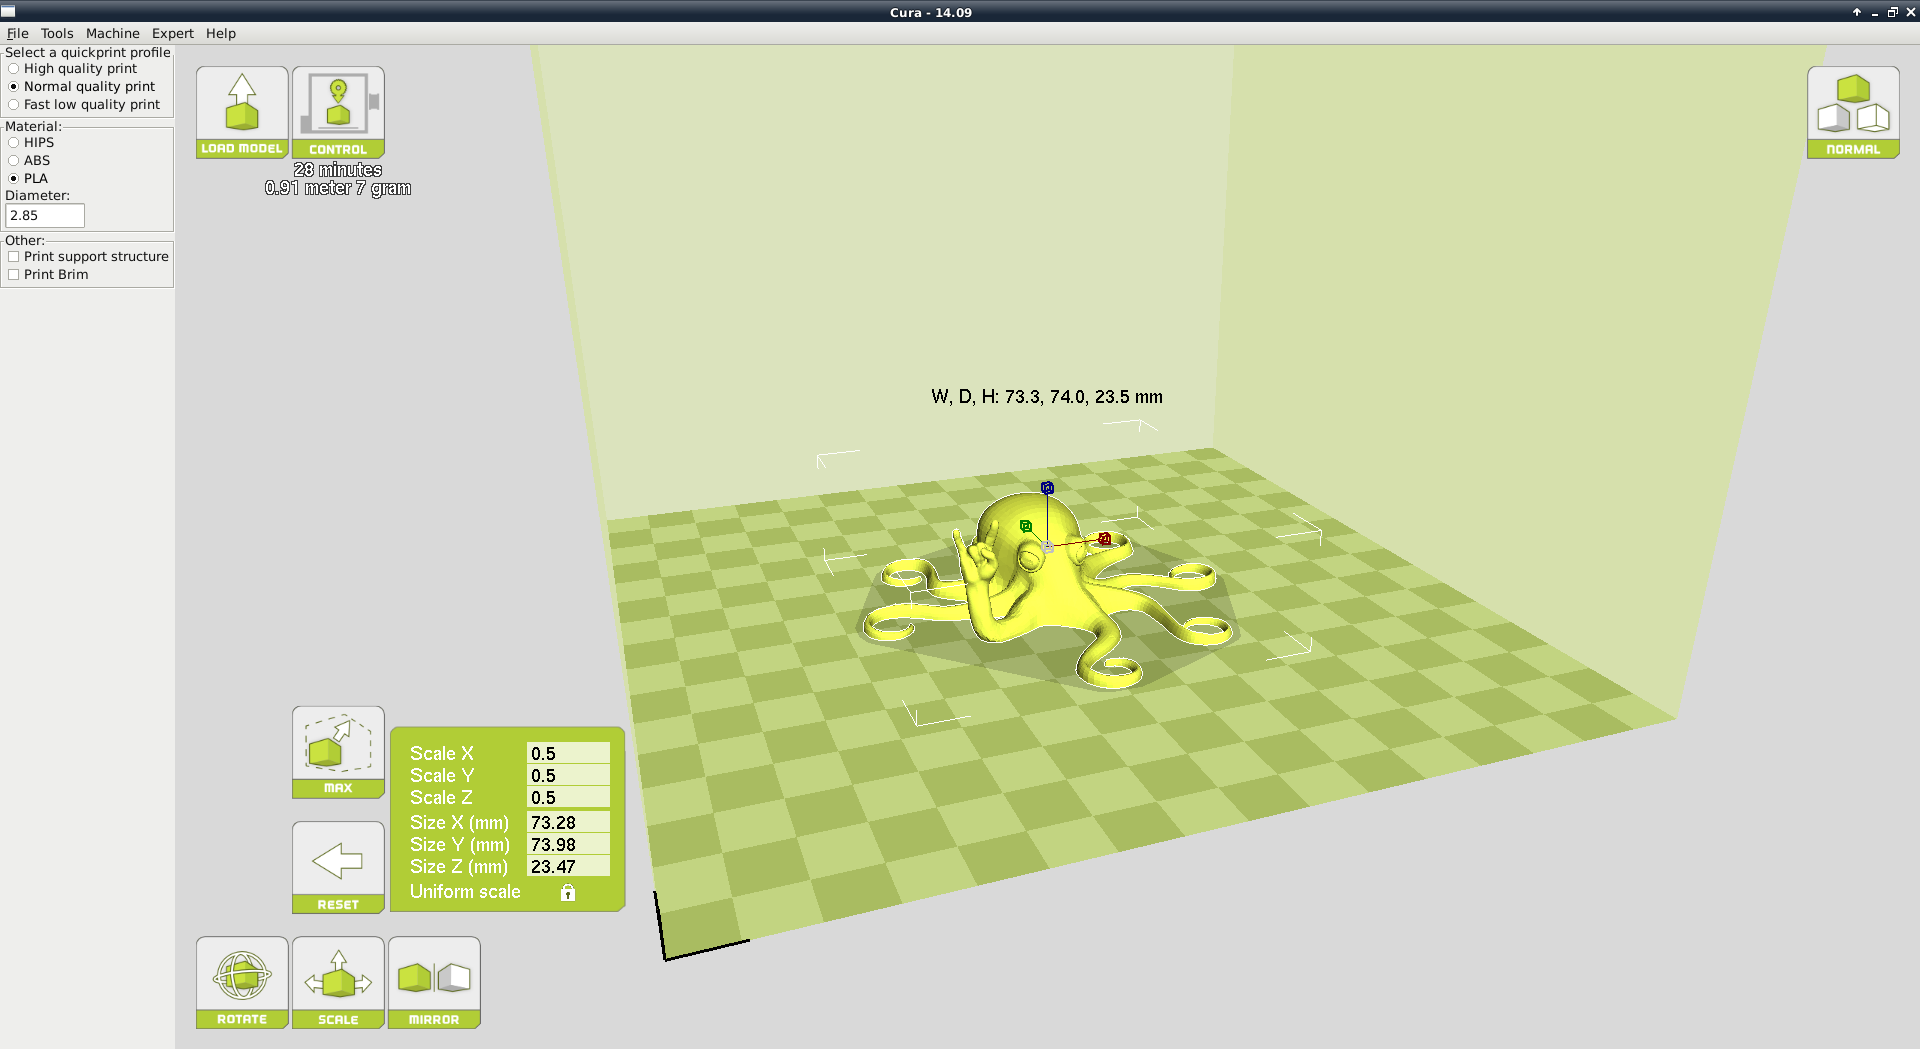
\includegraphics[keepaspectratio=true,angle=0,height=0.4\textheight,width=1.0\textwidth]{Scale.png}
\caption{Scaling your Model}
\label{fig:Scaling your Model}
\end{figure}

\section{View Mode}
\index{View Mode}

This will allow you to view your model in a variety of ways. This can be helpful for spotting issues before the print even starts. 

\subsection{Normal}
This is the standard setting for mesh files. It will show you the solid outer surfaces of your model file. 

%%%%%%%%%%%%%%%%%%%%%%%%%%%%%%%%%%%%%%%%%%%%%%%%%%%%%%%%%%%%%%%%%%%%%%%%%%%%%%%%

%\pageref{fig:Rotating}).
\begin{figure}[hbt]
\centering
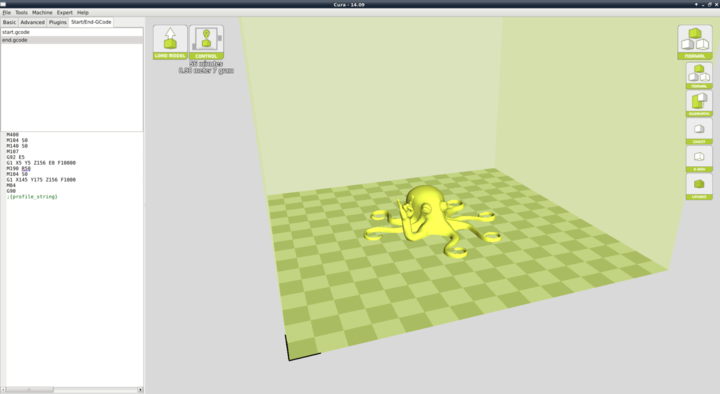
\includegraphics[keepaspectratio=true,angle=0,height=0.4\textheight,width=1.0\textwidth]{View.png}
\caption{View in Normal Mode}
\label{fig:Normal View}
\end{figure}

\subsection{Overhang}
\index{Overhang} 

Overhang mode will show where your print will have issues due to printing angle in mid air. In the photo below, you can see the red highlighted areas. These showcase where the angle in relation to the bed is between 0 and 30 degrees. It may be best to use support if your model has these areas.
% (overhang photo)

%\pageref{fig:Rotating}).
\begin{figure}[hbt]
\centering
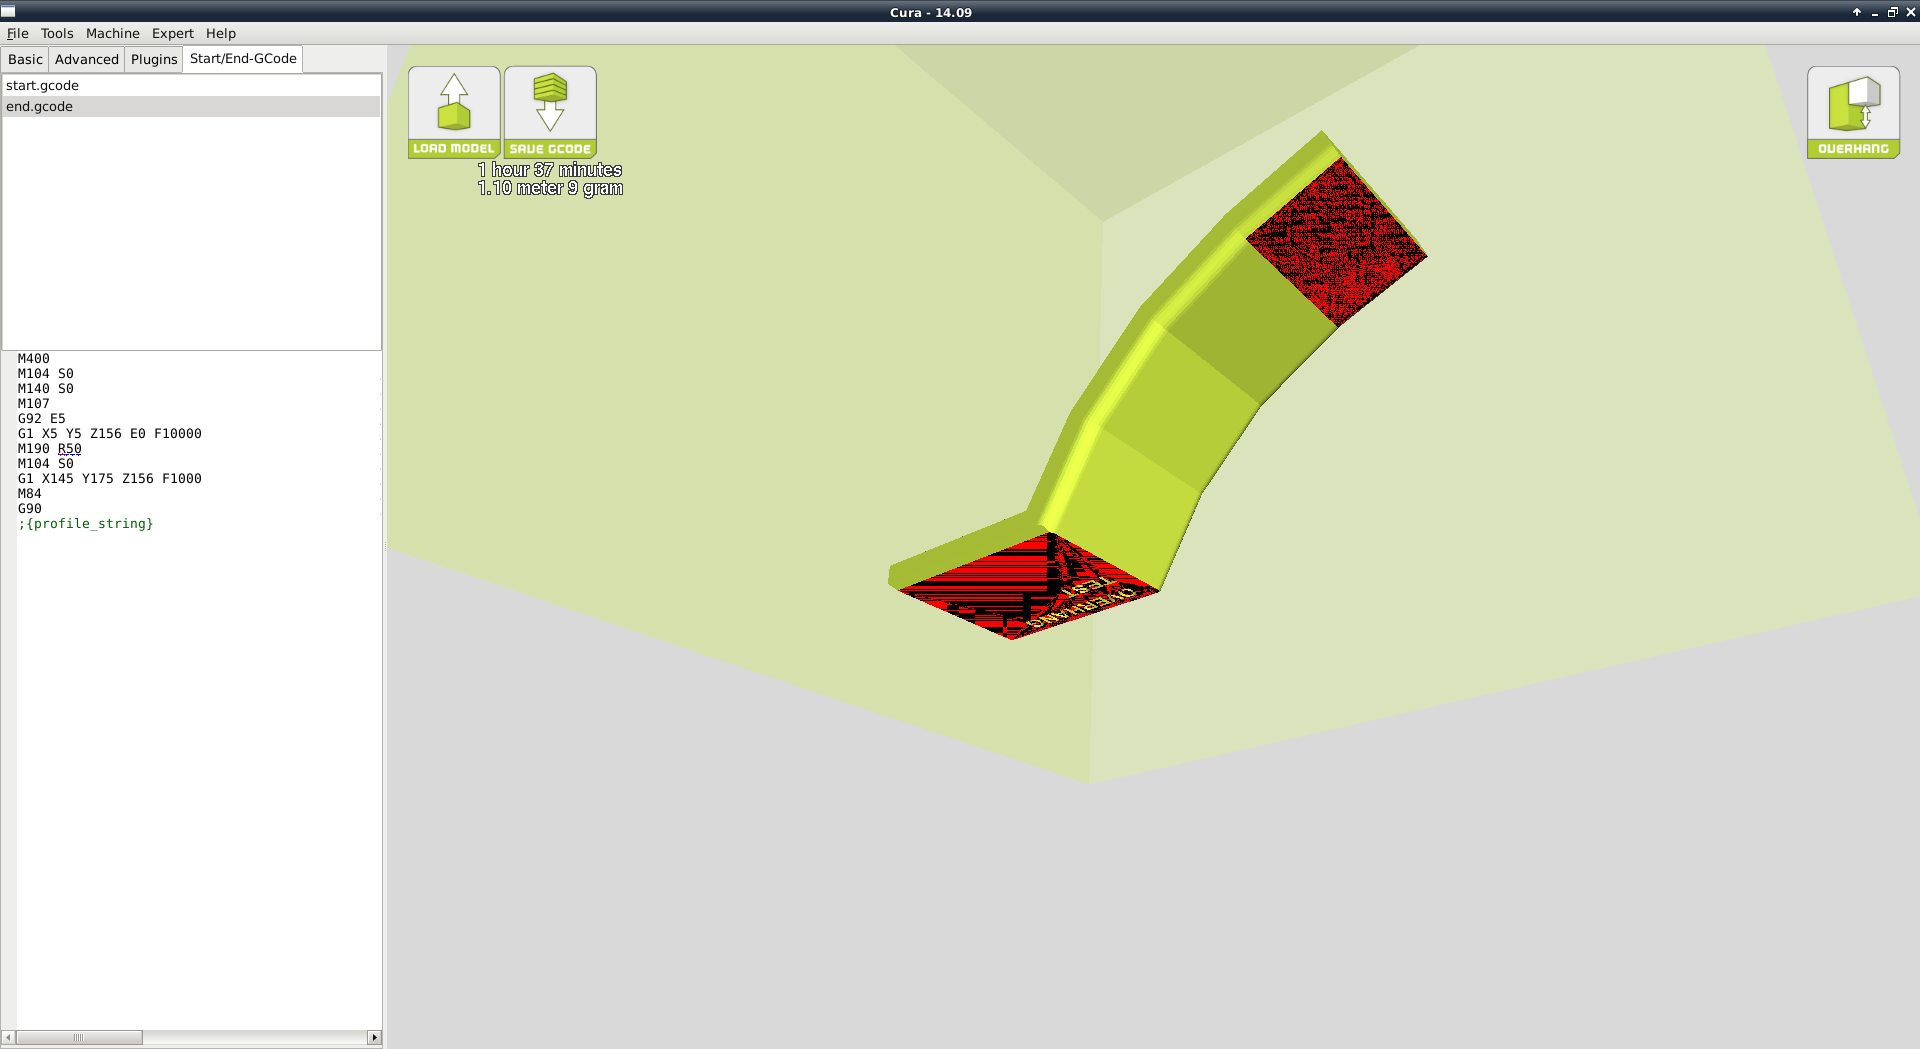
\includegraphics[keepaspectratio=true,angle=0,height=0.4\textheight,width=1.0\textwidth]{overhang.png}
\caption{View in Overhang}
\label{fig:Overhang View}
\end{figure}

\subsection{Ghost}
\index{Ghost}

Ghost view mode, will allow you to see through your model to what is behind it. This can be helpful for ensuring your entire model has loaded properly.
% (Ghost photo)
%\pageref{fig:Rotating}).
\begin{figure}[hbt]
\centering
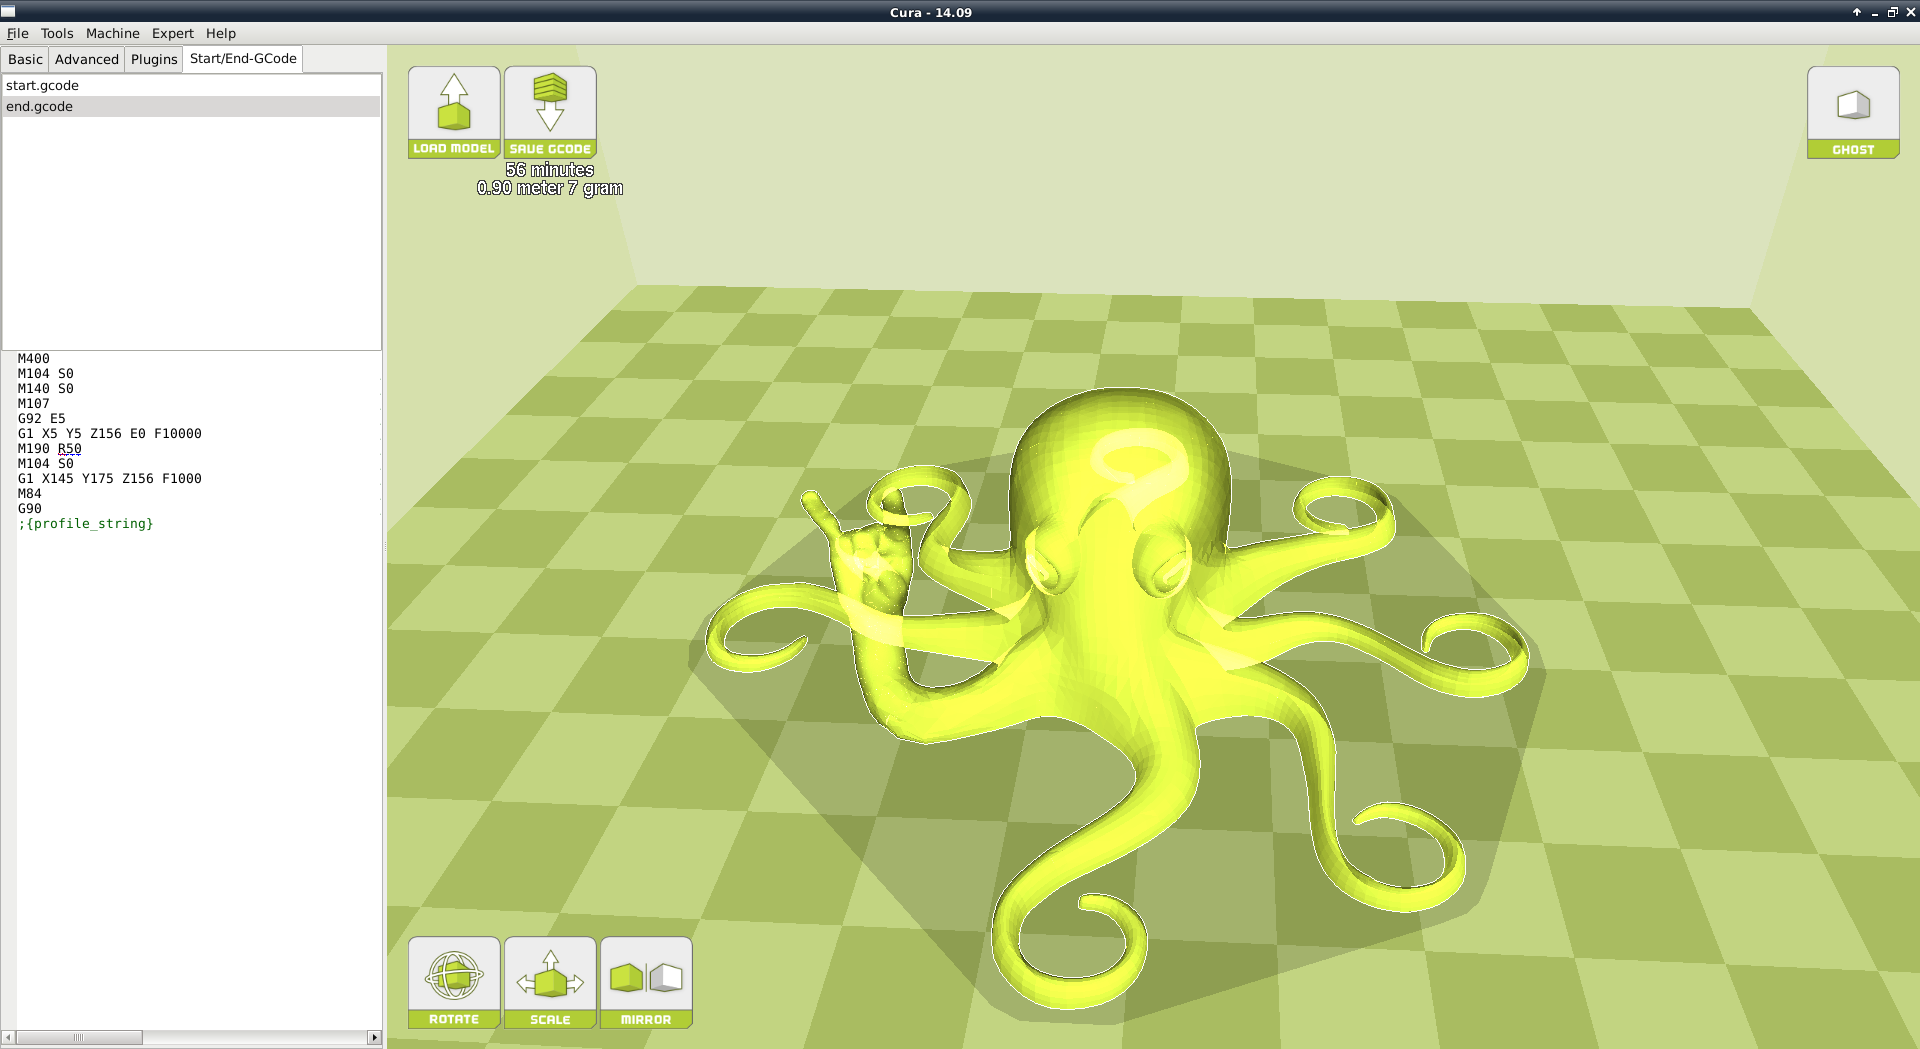
\includegraphics[keepaspectratio=true,angle=0,height=0.4\textheight,width=1.0\textwidth]{Ghost.png}
\caption{View in Ghost}
\label{fig:Ghost View}
\end{figure}

\subsection{Xray}
\index{Xray}

Xray is very similiar to ghost mode. It will alow you to see into objects, ensuring inner details are correct.
% (Xray2 photo)
%\pageref{fig:Xray}).
\begin{figure}[hbt]
\centering
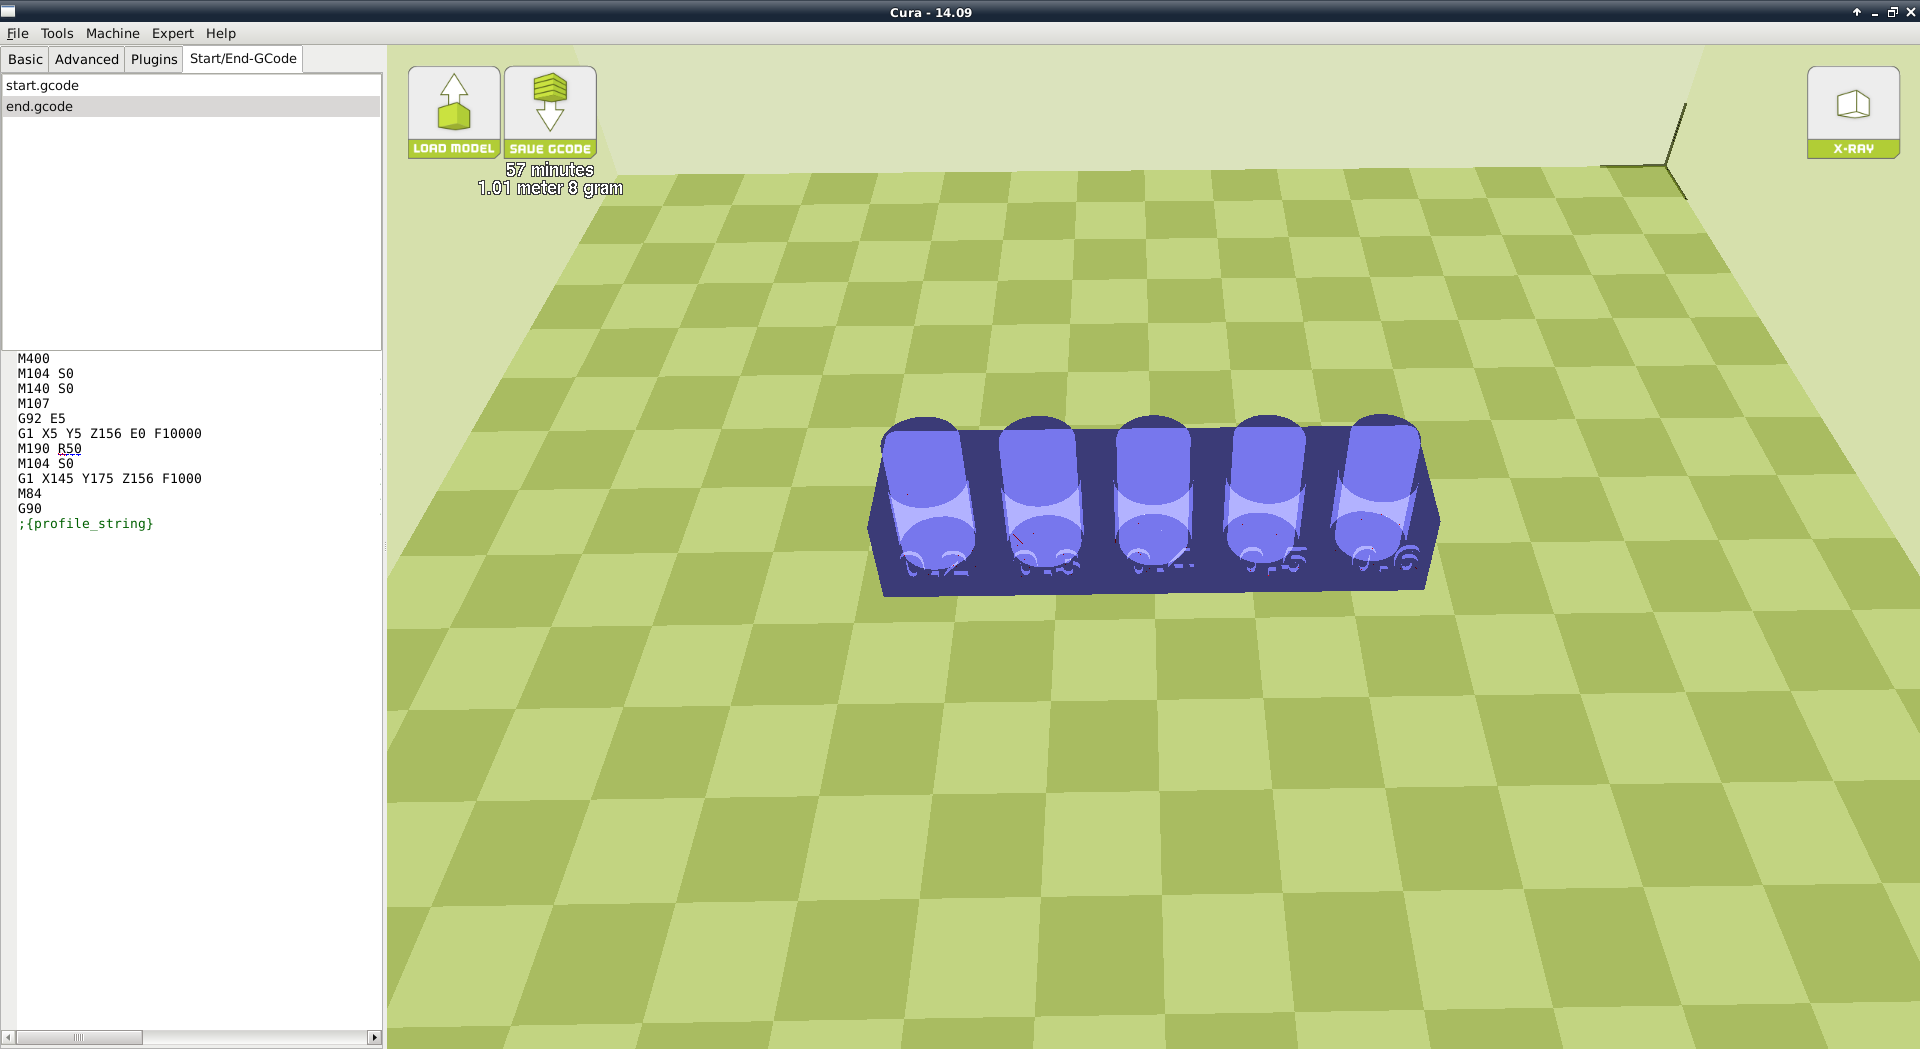
\includegraphics[keepaspectratio=true,angle=0,height=0.4\textheight,width=1.0\textwidth]{Xray2.png}
\caption{View in Xray}
\label{fig:Xray View}
\end{figure}

\subsection{Layers}
\index{Layers}

This will be the most helpful option for double checking prints. This will allow you to view the toolpath of your print head, to ensure to skipped layers or gaps. On the right hand side of your screen, you will see a slide bar. This will move up and down to view your desired layer.
% (Both layer photos)
%\pageref{fig:Layers}).
\begin{figure}[hbt]
\centering
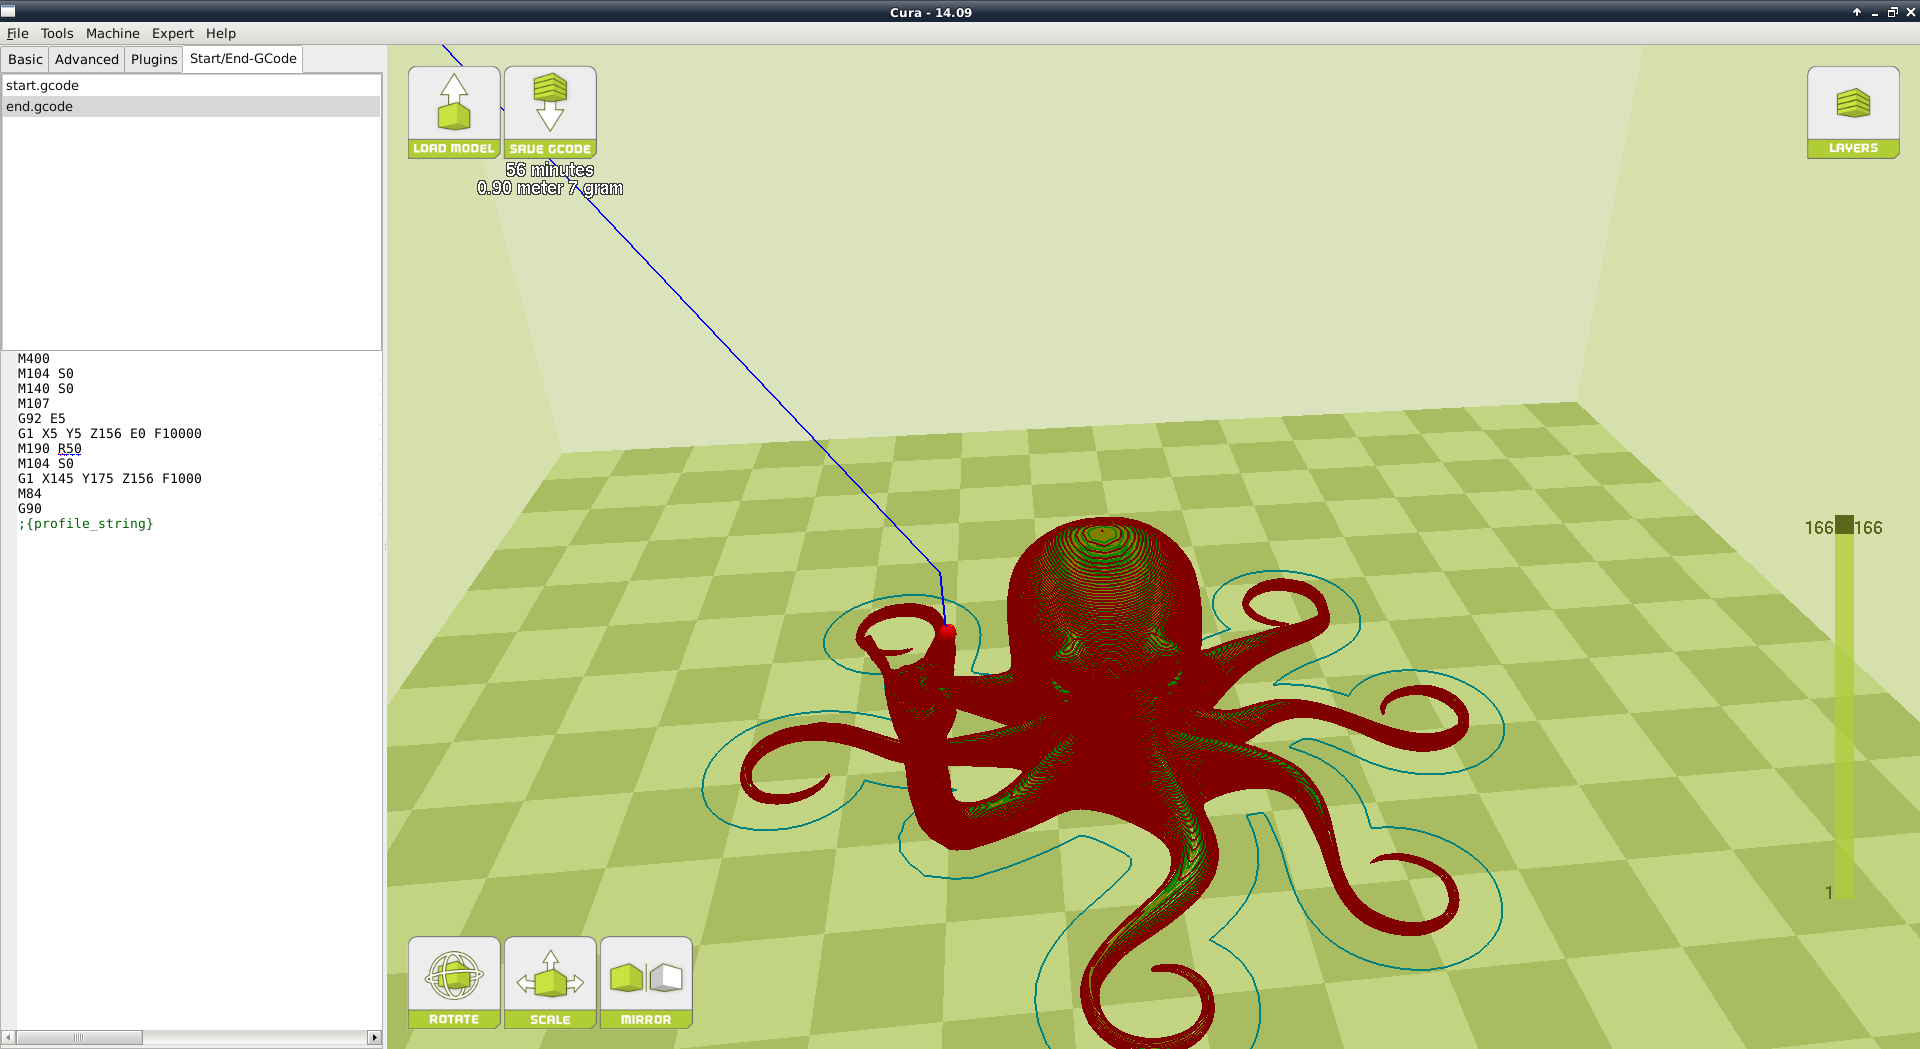
\includegraphics[keepaspectratio=true,angle=0,height=0.4\textheight,width=1.0\textwidth]{layers.png}
\caption{View in Layers}
\label{fig:Layers View}
\end{figure}
\pageref{fig:Mid Layers}).
\begin{figure}[hbt]
\centering
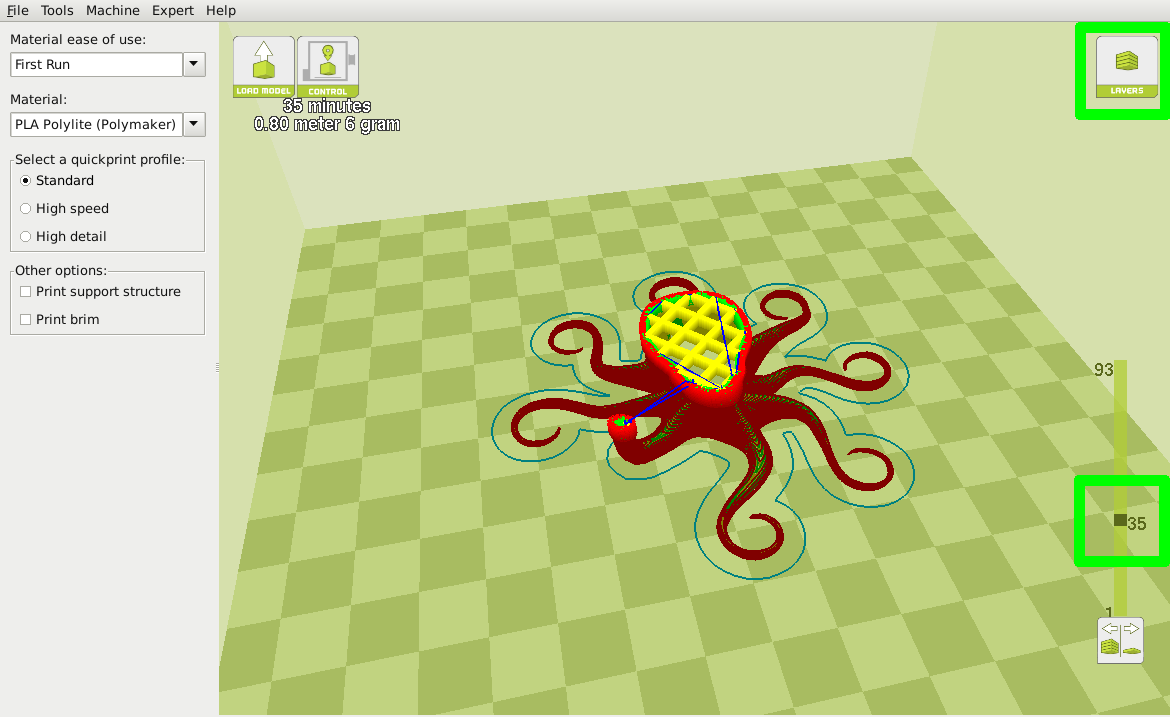
\includegraphics[keepaspectratio=true,angle=0,height=0.4\textheight,width=1.0\textwidth]{layers2.png}
\caption{View in Layers}
\label{fig:Mid Layers View}
\end{figure}

\section{Starting Your First Print}
\index{First Print}

Once you have your model, profile, and filament loaded, it is time for your first print! 

\subsection{TAZ Mini}

Select the Print/Control option in the top left hand corner of your build volume. This will bring up your Pronterface user interface. Please wait for the window to state “operational” before sending any commands to the printer. As soon as it is operational, all you need to do is hit print! This will allow your printer to set it's temperatures, go through the auto leveling procedure, and start laying down plastic.
% (print control photo)
%\pageref{fig:Print Control}).
\begin{figure}[hbt]
\centering
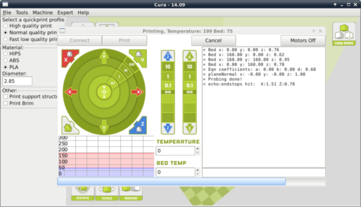
\includegraphics[keepaspectratio=true,angle=0,height=0.4\textheight,width=1.0\textwidth]{print_control.png}
\caption{Print Control Screen}
\label{fig:Print Control}
\end{figure}

\subsection{TAZ}

TAZ users will need to decide if they want to print directly from their computer using the USB cable, or if they would like to print from their SD card. 

\subsubsection{Printing from USB Cable}
\index{Printing from USB}

Once your printer is connected through the USB cable, please select the Print/Control button. This will bring up the Pronterface UI (photo). You will not be able to send any commands until the new box is titled “operational.” Once it is, you will need to set your temperatures for the hot end and the bed. You will see two boxes, one labeled “Temperature” and one labeled “Bed Temp”. Temperature will set your hot end, and bed temp will set your bed. Once your hot end and bed have reached temperature, you will just need to select print.
% (print control photo or reference above?)

\subsubsection{Printing from SD Card}
\index{Printing from SD}

You will need to save your Gcode file to your SD card. To do this, please go to File > Save Gcode > (select SD card). After putting the Gcode file to the SD card, you will need to insert it into the printer. Please be sure the metal tabs are facing forward. 

You will then need to pre heat your printer. You can do this for ABS and PLA by going to Prepare > Preheat ABS/PLA. If you are using other filaments, you can set your temperatures by going to Control > Temperature > Nozzle/Bed > (set specific temps). Then wait for printer to reach specified temps.
% (Reference LCD section in manual?)

Once heated, you can begin your print through your LCD by going to Print From SD >  (Select Desired File).

\section{Removing Your First Print}
\index{Removing a Print}

After your first print has finished, you will want to remove it from your bed. Your parts will be easier to remove if you allow your heated bed to cool down completely before removing the part. This will allow the plastic to contract, making it easier to remove.

Once your heated plate has cooled, you will want to use the blue clam knife that was included with your printer. Carefully use the clam knife to get between your print and heated bed. Once underneath the part, you can rotate the blade to pop the part off your plate.

\section{Full Settings}
\index{Full Settings}

When first starting Cura, you will be in QuickPrint settings. In order to have more control of your Gcode generation, you will need to switch to full settings. To do so you will need to go to Expert > Switch to full settings. This will give you access to the Basic, Advanced, Plugins, and Start/End-Gcode Tabs as well as access to the Expert Settings. % (expert photo)
%\pageref{fig:Expert Options}).
\begin{figure}[hbt]
\centering
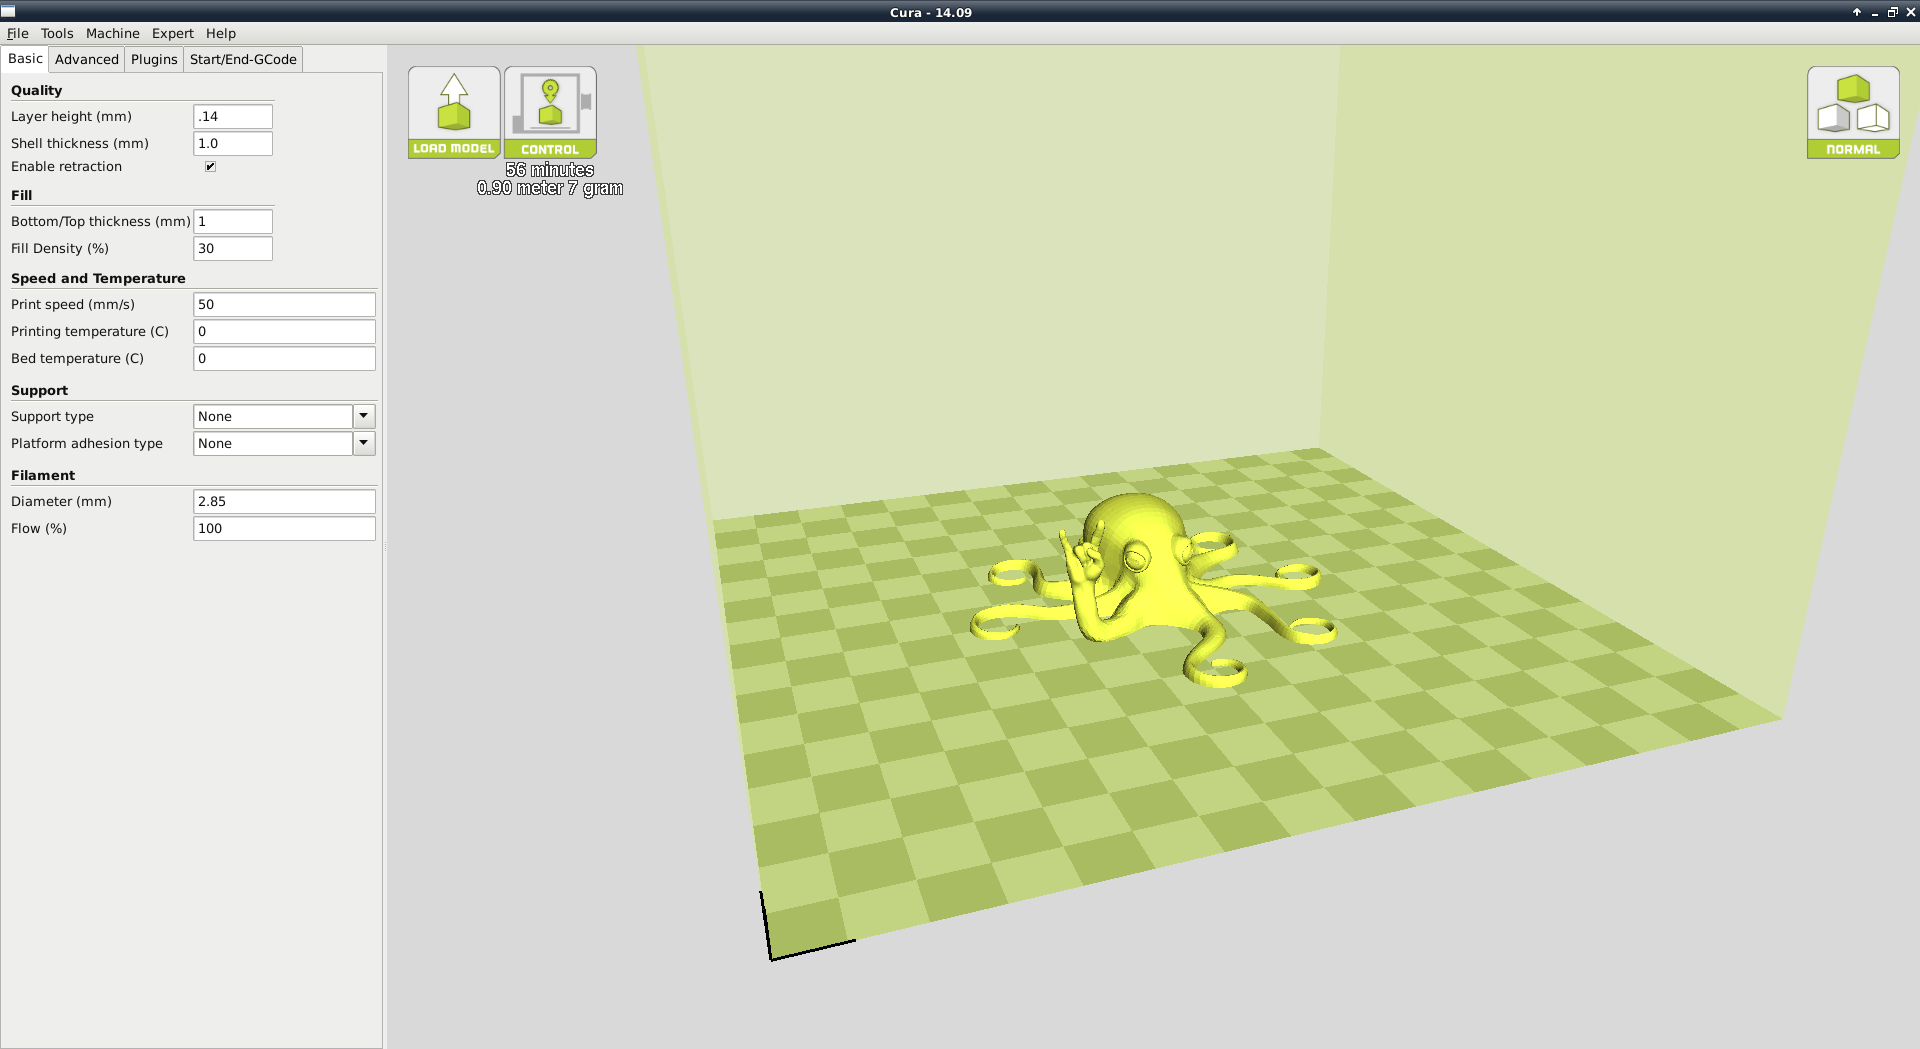
\includegraphics[keepaspectratio=true,angle=0,height=0.4\textheight,width=1.0\textwidth]{Expert.png}
\caption{View in Full Settings}
\label{fig:Full Settings View}
\end{figure}

\subsection{Loading a Profile}
\index{Loading Profile}

When you first switch to Full Settings, Cura will revert to very generic settings. We recommend when first starting to use one of our premade profiles that can be downloaded from here: \texttt{https://www.lulzbot.com/support/downloads} You will want to choose the profile that matches your filament and quality needs. Once downloaded, you can load the file into Cura by going to File > Open Profile > (Select). This will automatically update all of your settings for use with your printer.

\section{Basic Tab Options}
\index{Basic Options}

\subsubsection{Layer Height}
\index{Layer Height}

This will determine how thick each layer is. The smaller the layer height, the smoother curves will appear. Larger layer heights are better for bridging and overhangs. Smaller layer heights will also increase print time, as it will take more layers to complete the object. % (Layer height comparision photos)

\subsubsection{Shell Thickness}
\index{Shell Thickness}

This will define the number of vertical walls that follow the outside of your model. We recommend keeping this in multiples of your Nozzle width. The TAZ ships with a .35mm nozzle standard, while the TAZ Mini has a .5mm nozzle standard.

\subsubsection{Enable Retraction}
\index{Retraction}

This allows your printer to pull filament out of the hot end upon travel moves. We recommend keeping this on for all filament types, and adjusting the retraction length and speed for the specific filament. (Details given in advanced tab section. ((Reference?))

\subsubsection{Bottom/Top Thickness (mm)}
\index{Bottom Thickness}
\index{Top Thickness}

This will determine the number of of solid top and bottom layers. A larger number here will create a thicker top and bottom, which can be helpful for strength and quality purposes. We do recommend keeping this number as a multiple of your layer height.

\subsubsection{Fill Density}
\index{Fill Density}

This number will relate to a percentage. 0\% will give a completely hollow print, while 100\% will give you a completely solid object. We have found that 20\% to 40\% fill density is functional for most prints.

\subsubsection{Print Speed (mm/s)}
\index{Print Speed}

This will be your overall printing speed. If no other speeds are determined in other sections, your printer will automatically default to this speed. 

\subsubsection{Printing Temperature}
\index{Printing Temperature}

We recommend leaving this temperature setting to “0”. If you set your temperature in this section, it can take 45 minutes or more for your printer to start. You will set your printing temperatures through your printing program, or through your LCD.

\subsubsection{Bed Temperature}
\index{Bed Temperature}

We recommend leaving this temperature setting to “0”. If you set your temperature in this section, it can take 45 minutes or more for your printer to start. You will set your printing temperatures through print control, or through your LCD.

\subsection{Support Type}
\index{Support Type}

Some models will require support in order to print properly. This will usually occur when an object has an angle, in relation to the build plate, between 0 and 45 degrees. It is highly recommended to orient your object as such that it minimizes, or eliminates the need for support.

\subsubsection{Touching Buildplate}

This will cause the support material to build up between the plate and the object only. (Photo of Circle inside a square, that is printed vertically. Have samples on photo table)

\subsubsection{Everywhere}

This will cause support material to be created between the bed and object, and also between the object and itself. (Photo of Circle inside a square, that is printed vertically, sample on photo table)

\subsection{Platform Adhesion Type}
\index{Adhesion Type}

Some models have a small surface area contacting the plate. This can create adhesion issues, allowing your part to pop off at some point during the print. To fix this, you can add either Brim or a Raft to your STL.

\subsubsection{Brim}
\index{Brim}

Brim will create a single layer of filament, contacting and surrounding your model. This will increase the surface area of the STL contacting the build platform, preventing it from popping off. Brim will also help in situations where you are seeing corner lift. Brim is defined in expert settings. (See Expert Settings/Page REFERENCE)

\subsubsection{Raft}
\index{Raft}

Will generate a layer of material underneath your object. This will help ensure a perfectly flat layer. Raft was more often used before the addition of heated plates, but may still be helpful. You can define how the raft is generated in expert settings. (See Expert Settings/Page REFERENCE)

\subsection{Filament Diameter}
\index{Filament Diameter}

The filament diameter setting will be your true filament diameter. Although your filament will say 3mm, it is more likely going to be near 2.9mm +/- 0.1mm. You will want this to be a true average, as it will allow your printer to accurately calculate how much filament it is extruding. If you are using non Lulzbot brand filament, please update this to your true average.

\subsection{Filament Flow \%}
\index{Flow Rate}

This will control how much filament your printer is putting out in relation to speed. The TAZ and TAZ Mini will come from the factory already calibrated. Please leave this number at 100\% as changing it can lead to surface quality issues.

\section{Advanced Tab Options}
\index{Advanced Options}

\subsection{Nozzle Size (mm)}
\index{Nozzle Size}

This will define your Nozzle size. Your printer will use this combined with your other settings to determine how quickly to feed filament into your nozzle. The TAZ ships with a 0.35mm nozzle, and the TAZ Mini ships with a 0.5mm nozzle.

\subsection{Retraction Speed (mm/s)}
\index{Retraction Speed}

This will determine the speed at which your filament backs out of the hot end for travel moves. We recommend keeping this set to 25mm/s. If you set this number above 30mm/s, you risk damaging your Herringbone Gears.

\subsection{Retraction Distance}
\index{Retraction Distance}

This will determine how much filament is pulled out of your hot end on travel moves. You will want to adjust this depending on temperature settings and filament type. Higher thermal retaining filaments behave better with a longer retraction distance. We have found anywhere from 1mm to 6mm is a good starting range.

\subsection{Initial Layer Thickness}
\index{Initial Layer}

This will control how thick your initial layer height is. Having a larger initial layer will help with bed adhesion.

\subsection{Initial Layer Line Width}
\index{Initial Layer Width}

This will control how wide your first layer will be. As with initial layer height, a wider line will help with bed adhesion. We have found 125\% to be a good starting place.

\subsection{Cut Off Object Bottom (mm)}
\index{Cut Off Object}

This setting is used to help print models that were not specifically designed for FDM printing. Specifically, it is for STL's that do not have a flat surface to adhere to the plate. It will sink your object Xmm into the build plate, creating a nice flat surface to begin your print. (*Note* You will not be able to print the part of the object that is sunk into the platform. *Note*)
%\pageref{fig:Cutoff Setting}).
\begin{figure}[hbt]
\centering
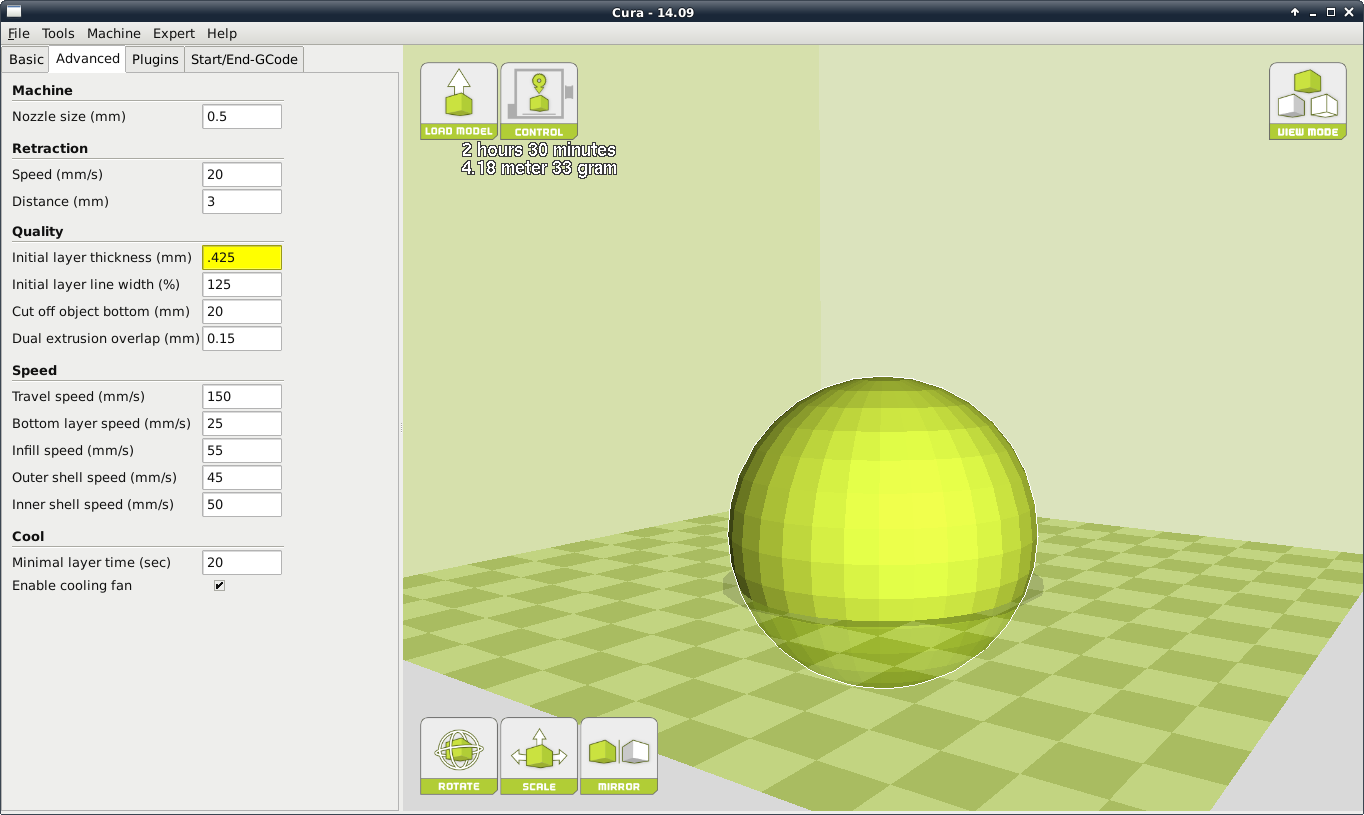
\includegraphics[keepaspectratio=true,angle=0,height=0.4\textheight,width=1.0\textwidth]{cutoff.png}
\caption{Cutoff Example}
\label{fig:Cutoff Example}
\end{figure}

\subsection{Dual Extrusion Overlap}
\index{Dual Extrusion Overlap}

This will determine how far your Dual Extruders will overlap when laying down material. This will help adhesion between the two different colors or types of filament. (You can ignore this setting unless you have installed the dual extruder upgrade.)

\subsection{Travel Speed}
\index{Travel Speed}

This setting will determine how fast your print head moves while not extruding filament. The TAZ and TAZ Mini will have no problem at 175mm/s when not printing.

\subsection{Bottom Layer Speed}
\index{Bottom Layer Speed}

This will control your initial layer speed. In general, a slower initial layer speed will help with first layer adhesion. 

\subsection{Infill Speed}
\index{Infill Speed}

This will control how quickly your print head moves while laying down the filler of your model. Faster speeds are usually tolerable here, as none of infill will be visible on the outside of your object. If you go too fast compared to your inner and outer shells, you can have adhesion issues.

\subsection{Outer Shell Speed}
\index{Outer Shell Speed}

This will be the outermost vertical shell from the Basic settings. This is the most important setting, as it controls the speed of your print head on the visible layers. As a general rule of thumb, the slower you go the better looking print you will get. 

\subsection{Inner Shell Speed}
\index{Inner Shell Speed}

This will be the vertical walls, that are in between the outer shell,         and infill. This will not be visible, but will help support the outer shell and the infill. We recommend keeping this speed setting between your infill and your outer shell speed to help adhesion.

\subsection{Minimal Layer Time}
\index{Minimal Layer Time}

This will determine a minimum amount of time your print will spend laying down one layer. If your print time is below this, your printer will automatically slow down to reach this time, before moving onto the next layer. This will never reduce your printing speed below the minimum time. (See Expert Settings/Page REFERENCE)

\subsection{Enable Cooling Fan}
\index{Enabling Cooling Fan}

This will allow operation of your extruder's active cooling fan. You can control how the fan operates by adjusting the cooling settings in expert options. (See Expert Settings/Page REFERENCE)

\section{Plugins}
\index{Plugins}

Plugins are custom settings which will alter your print at specific points. The two that come pre loaded with Cura are Tweak at Z, and Pause at Height. More plugins and information can be found here: \texttt{http://wiki.ultimaker.com/Category:CuraPlugin} To activate one of these, you will need to highlight the desired plugin, and click the down arrow directly below the Plugins box. (photo Plugins)
%\pageref{fig:Plugins}).
\begin{figure}[hbt]
\centering
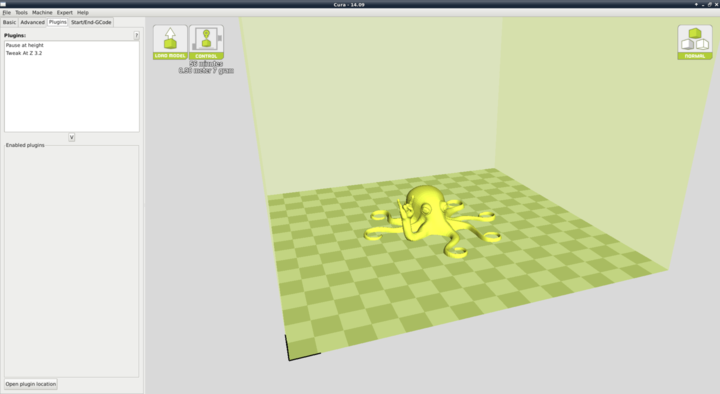
\includegraphics[keepaspectratio=true,angle=0,height=0.4\textheight,width=1.0\textwidth]{Plugins.png}
\caption{View of Plugins}
\label{fig:Plugins}
\end{figure}

\subsection{Tweak at Z}
\index{Tweak at Z}

This will allow you to make basic changes at specified Z heights. You can determine the Z height or layer count at which you want to make a change. Then choose how you would like to change your settings. You can alter temperatures, fan speeds, and print speeds.

\subsection{Pause at Z Height}
\index{Pause at Z Height}

This will pause your print at a specified height. You can also specify where         to move the print head, and how much filament to retract. This will prevent “blobs” from accumulating on your print while paused. This setting is most commonly used when switching colors of filaments in the middle of a print.

\section{Start and End Gcode Settings}
\index{Custom Gcode}

This is where you can make custom settings to your print profiles. By adding custom Gcode into the start or end of your file, you can alter how it prints. A comprehensive list of Gcode commands can be found here: \texttt{http://reprap.org/wiki/G-code} We recommend new users to leave this as provided in the profiles at \texttt{https://www.lulzbot.com/support/downloads}

\subsection{TAZ Mini}
Please be cautious when changing any of these start and end gcode settings. This is where your Auto Bed Leveling commands are stored. If improperly altered, your printer will no longer         automatically bed level. If you are uncertain of the change you are trying to make, please contact us at \texttt{Support@lulzbot.com} before hand.

\section{Expert Settings}
\index{Expert Settings}

Expert settings will give you more specific options for your retraction, skirt, active cooling, infill, support, brim, raft, and special settings. To gain access to this section you can go to Expert > Open Full Settings or you can hit Control + E. (Photo expert)
%\pageref{fig:Expert Settings}).
\begin{figure}[hbt]
\centering
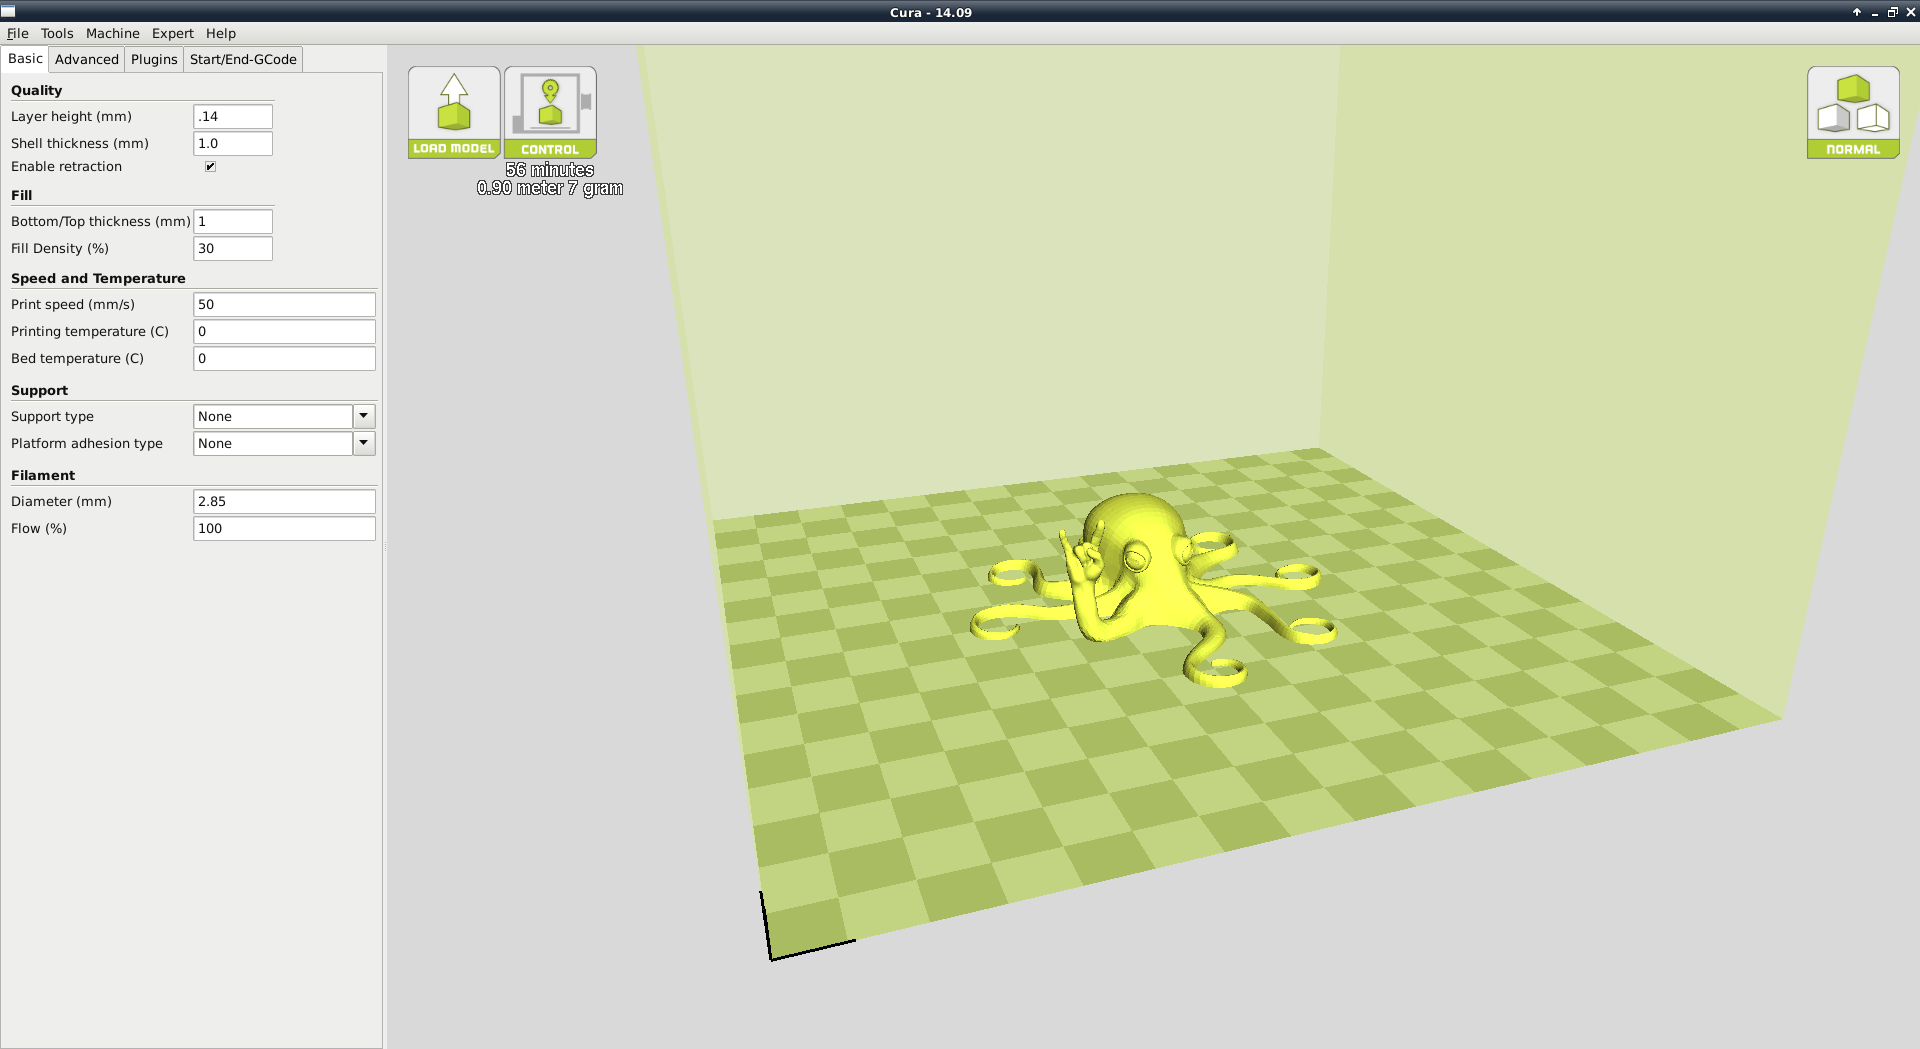
\includegraphics[keepaspectratio=true,angle=0,height=0.4\textheight,width=1.0\textwidth]{Expert.png}
\caption{View Expert Settings}
\label{fig:Expert Settings}
\end{figure}

\section{Retraction}
\index{Retraction}

Retraction pulls filament out of your nozzle when it is not extruding to prevent your print head from dripping on your object.This section is where you will control how and when your extruder retracts its filament.

\subsection{Minimum Travel}
\index{Minimum Travel}

This sets the minimum travel distance of your printhead in order to retract. If your print head is not moving this far during dravel moves, it will not retract.

\subsection{Combing}
\index{Combing}

This option prevents your print head from traveling over holes in the X/Y plane when printing. This will slightly increase print time, but will prevent strings from getting caught on the holes during travel moves.

\subsection{Minimal Extrusion Before Retracting}

This will put a minimum extrusion amount before retracting. This will prevent a retraction move, if your extruder has not put out Xmm of filament since its last retraction.

\subsection{Z Hop When Retracting}
\index{Z hop}

This will raise your print head Xmm while retracting. This setting helps prevent ooze, and strings from being deposited on your print. (*Note* We do not recommend this setting for TAZ 3 users and earlier. This can cause issues with Z dimensional accuracy. *Note*)

\section{Skirt}
\index{Skirt}

Skirt creates a line around the outside of your object. Most commonly used to prime the extruder, in order prevent missed filament at the beginning of a print.

\subsection{Line Count}
\index{Line Count}

This will define the number of loops the Skirt creates around the outside of your object. Smaller models will require more loops to properly prime the extruder.

\subsection{Start Distance}
\index{Start Distance}

This will define the distance away from your STL that the skirt will be created. If using as an envelope to prevent drafts, it is recommended to be closer to your object.

\subsection{Minimal Length}
\index{Minmal Length}

This will define the minimum amount of filament to be pushed into your hot end for the skirt. This will over ride your line count, producing as many lines as required to reach the minimal length.

\section{Cool}
\index{Cooling}

This section will define how your extruder cooling fan will operate during the print. \texttt{(*Note* Your fan will not start until it has reached 25\% or higher for speed settings. *Note*)} If your print speeds are slowed down due to minimal layer time, the fan will run between minimum and maximum speed based upon how much the layer is slowed down.

\subsection{Fan on at Full Height}
\index{Fan Settings}

This is your Z height where your fan will be turned to its maximum percentage. Especially helpful with high temperature retaining filaments such as PLA. This will be scaled between 0\%, and your maximum fan speed based upon layer height with it being disabled for the first layer.

\subsection{Fan Speed Min}
\index{Fan Settings}

This will be the minimum fan speed when enabled. If fan on at full height is enabled, this will be the minimum speed and it will scale to the maximum speed at that height.

\subsection{Fan Speed Max}
\index{Fan Settings}

This is the fastest speed at which your will ever run. When Fan on at Full Height is enabled, this is the speed at which it will be set.

\section{Support}
\index{Support Material}

You define how your support is generated here. You must have some form of support turned on in the basic settings in order for these settings to have an effect.

\subsection{Structure Type}
\index{Support Settings}

You can choose between a Grid or a Line pattern for your support material. The grid will be a checkerboard pattern, in the X and Y direction. The line option, will just give lines in the Y direction for support. The grid will provide better support the line option, but will be harder to remove.

\subsection{Overhang Angle for Support}
\index{Overhang Angle}

This will determine where support material is generated. The TAZ and TAZ Mini will be able to print 45 to 90 degree angles in relation to the bed without support. We recommend leaving this setting at 45.

\subsection{Fill Amount}
\index{Fill Amount}

This will determine how solid your support material is. That is, how close together your support lines are. The higher percentage the better support, but it will be harder to remove the support material and will use more material.

\subsection{Distance X/Y}
\index{Support}

This will determine how far away from your object in the X/Y plane that the support material is being placed. You will want to adjust this to optimize each particular STL you are printing.

\subsection{Distance Z}
\index{Support}

This will determine how far away your support material is from your object in the vertical direction. A smaller number here makes for better support, but makes it harder to remove. Adjusting this for each individual STL is also recommended.

\section{Black Magic}
\index{Black Magic}

This section allows you to transform your STL into a hollow shell, a single layer thick. (*Note* May not be possible for all models. *Note*)

\subsection{Spiralize the Outer Contour}
\index{Spiralize}

This causes your Z axis to be constantly moving upward as printing your single outer wall shell. The results are no layer change lines, giving a much smoother surface.

\subsection{Only Follow Mesh Surface}
\index{Black Magic}

This will cause your print to follow the outside of your STL, building it completely hollow with a single wall outer shell. The only difference between this and Spiralize, is that the Z axis moves regularly. That is, it prints a layer and then moves up to the next one.

\section{Brim}
\index{Brim}

Brim circles the base of the print while making contact, helping adhere the print to the heated plate. This is only one layer thick, and easily removed post print. This section defines how the brim is formed. (When brim is activated in basic settings.)

\subsection{Brim Line Amount}
This will determine the number of loops the brim will create around the outside of your object. The more lines, the better your part will adhere to the plate. 

\section{Raft}
\index{Raft}

Raft is a platform built underneath your object, designed to help adhesion and prevent warping. It will lay down support material, and then a platform on top of the supports. Your STL will be built on top of this platform. 

\subsection{Extra Margin}
\index{Extra Margin}

This determines the distance around the outside of your object that the raft is created. Can be helpful for ensuring no warping of the lower layers.

\subsection{Line Spacing}
\index{Line Spacing}

This will determine the spacing between “support” lines for the raft. A small spacing makes the support structures closer together improving strength of the raft, but uses more material.

\subsection{Base Thickness}
\index{Base Thickness}

This defines how thick your raft will be. We have found that 0.5mm seems to be a good starting point.

\subsection{Base Line Width}
\index{Base Line Width}

This will define how wide your “support” material is for the raft. This setting will determine how well the surface layers of the raft print.

\subsection{Interface Thickness}
\index{Interface Thickness}

This will determine how thick the surface layers of the raft are. The surface layers are the platform that is built upon the supports.

\subsection{Interface Line Width}
\index{Interface Line Width}

This will determine how wide the top layers of the platform will be. In general, you can keep this set to your nozzle size, as surface quality of the removable raft is not important.

\subsection{Airgap}
\index{Airgap}

This will define the distance between your raft and your STL. A larger gap will make your part easier to remove, but will make the bottom of your print looks worse.

\subsection{Surface Layers}
\index{Surface Layers}

This will determine the number of layers that create the “platform” of your raft. If you have a wide line spacing, you may want to increase this number to ensure a solid platform. 

\section{Fix Horrible}
\index{Fix Horrible}

These are some of the more advanced and experimental options. They are designed to help repair poor models, to make them suitable for 3D printing. As a note, they do not always work. Please be cautious when using these options, as they can have unintended effects on your print quality.

\subsection{Combine Everything (Type-A)}
\index{Combine Type-A}

This will attempt to fix all external mesh errors, while keeping internal holes in tact. This can mistake intentional internal holes, and fill them in.

\subsection{Combine Everything (Type-B)}
\index{Combine Type-B}

This will ignore all internal holes of the model, and only focus on the external holes. This is helpful when one only cares of the outside finish of the STL.

\subsection{Keep Open Faces}
\index{Open Faces}

This will ignore all manifold errors in the object. It can create issues generating the Gcode, as Cura does not know how to interpret the open holes. This option should only be used if you are sure that the holes in the mesh are intended. In general, you should not use this option.

\subsection{Extensive Stiching}
\index{Extensive Stiching}

This causes Cura to automatically add triangle meshes, in an attempt to fix manifold errors. This algorithm will greatly increase Gcode generation time, and may end up adding in un-intended mesh. It is recommended to repair your STL through Meshlabb or your CAD program before attempting this option.
